\subsubsection{Segmentation} \label{segmentation-subsubsec}

\todo[inline,color=green!40]{Verantwortlich: Artur \\
- Bereit zum Korrekturlesen.}

Ziel dieses Schrittes ist es, Teile von Daten zu identifizieren, welche wichtige Informationen über die zu erkennenden Emotionen enthalten. 
Dies geschieht durch Filtern der Daten und Ausschließen von Segmenten, die für das Klassifizierungsproblem nicht relevant sind.
Zusätzlich wird die zu verarbeitende Datenmenge reduziert, indem Segmente eines Zeitfensters fester Größe aus den Daten extrahiert werden.
Diese Vorgeheisweise ist heute in der Praxis besonders wichtig, da sonst hardwarebedingte Einschränkungen die zu verarbeitende Datenmenge begrenzen könnten. \\

\todo[inline]{Eventuell fehl am Platz, wenn hier nur Grundlagen und weitere Details erst später.\\
- Abklären.}

In dieser Projektarbeit wurde ein Schiebefensteransatz (engl. ``sliding window approach'') verwendet. 
Ziel der Methode ist die Segmentierung der vorhandenen Daten in kleinere Einheiten, um die Merkmalsextraktion sowie die anschließende Klassifizierung zu vereinfachen oder gar erst zu ermöglichen.
Die Länge des Zeitfensters (engl. ``time window'') und des Gleitschritts (engl. ``sliding stride'') sind zu bestimmende Parameter (und werden auch als ```Hyperparameter'' bezeichnet), wobei sich das Zeitfenster auf die feste Größe pro extrahiertem Segment und der Gleitschritt auf den Abstand zu dem Beginn des darauf folgenden Zeitfensters bezieht.
Es ist zu beachten, dass sich aufeinanderfolgende Zeitfenster überlappen können, sobald der definierte Gleitschritt kleiner als das Zeitfenster ist. \\


Die Daten werden auf Zeitstempel-Ebene mit Etiketten beschriftet, basierend auf den von der jeweiligen Versuchsperson ausgefüllten Fragebögen. 
Jedem Zeitfenster wird ein Etikett zugeordnet, welches das dominate (d.h. am meisten vohandene) Etikett der im entsprechendem Fenster enthaltenen Zeitstempel basiert. Es wird davon ausgegangen, dass jedes Zeitfenster nur von einer Emotion belegt ist. \\


\begin{figure}[h]
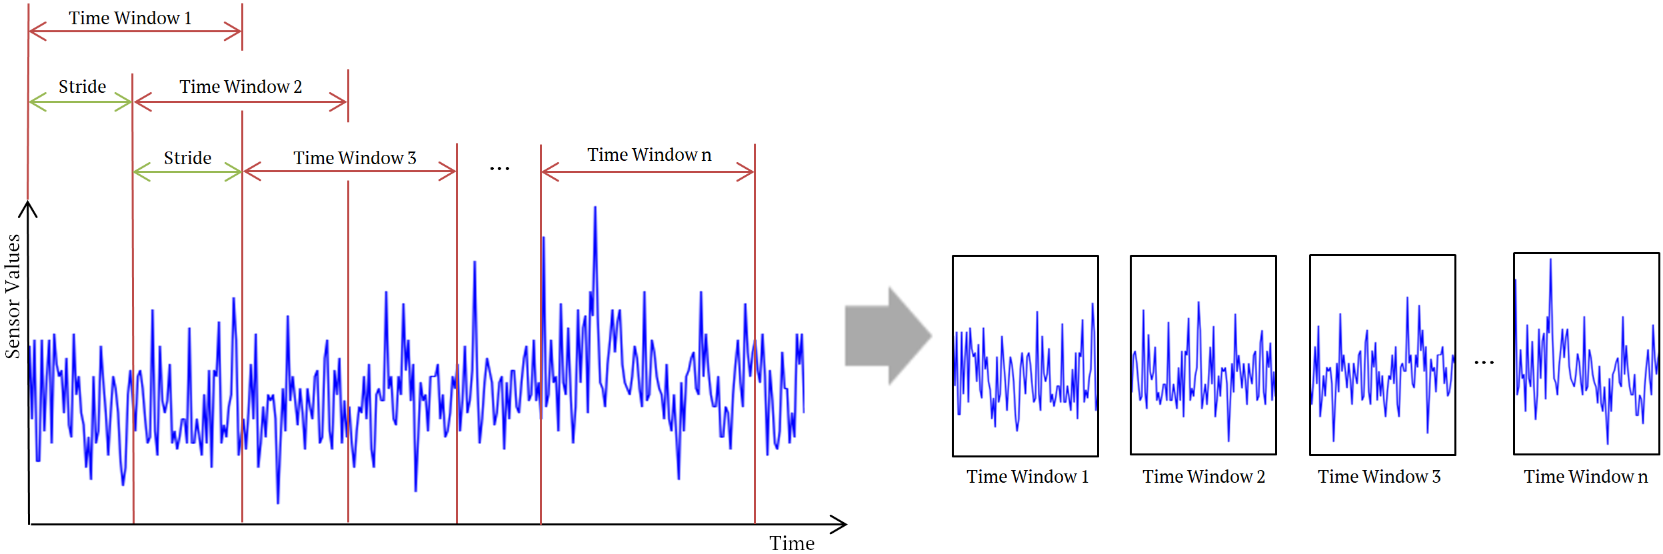
\includegraphics[width=\textwidth]{Images/segmentation.png} 
\caption[Schiebefenster-Segmentierung]{Schiebefenster-Segmentierung: Die Daten werden durch ein Zeitfenster fester Größe in kleinere Segmente aufgeteilt. Das Fenster wird mit einem festen Gleichschritt geschoben, um den aufeinanderfolgend Daten-Zeitfenster zu erhalten. }
\end{figure} 